\section{Performing a firmware update}

After installing the \deviceName\ device driver, a firmware update tool is available.
 By choosing ``FirmwareGUI.exe'' a firmware update can be performed. 
 After invoking the application, a window as shown in Figure \ref{fig:Firmware} will appear. 
 The tool can be used for updating the firmware and to create a backup of the on-board calibration data of the \deviceName\ unit. 
 If several boards are present, the one which is going to be used can be selected in the upper left corner of the window. 
 When pressing one of the ``Backup'' buttons a backup of the firmware or the calibration data will be created, respectively. 
 In order to perform a firmware update, chose the ``.cronorom''-file to be used by pressing ``Browse''. 
 The file contains the firmware data. By pressing ``Flash'' the firmware is written to the board. 
 ``Verify'' can be used to compare the firmware data stored on the \deviceName\ to the one inside a file.
 ``Flash All'' and ``Verify All'' perform the corresponding operation on all boards which are installed.\par

\begin{figure*}[ht]
    \begin{center}
        \itett{
            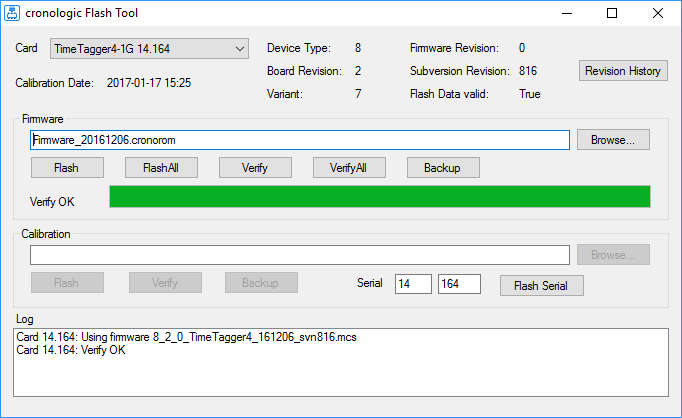
\includegraphics[width=0.8\textwidth]{figures/TT4_flashtool.png}
        }{
            \includegraphics[width=0.8\textwidth]{figures/xTDC4_flashtool.png}
        }
        \caption{\label{fig:Firmware}The firmware update and calibration data backup tool as provided with the \deviceName\ device driver.}
    \end{center}
\end{figure*}

\textbf{Important note:} The new firmware will only be used by the board after a power cycle, i.e. after switching the PC (or Ndigo crate) off and back on. 
A simple reboot is not sufficient. Therefore the information shown in the upper half of the application window does not change right after flashing a new firmware.

\itett{}{ %This section only for xTDC4
\section{Calibrating the Carry-Chain TDC}
After each update of the \deviceName\ firmware the Carry-Chain TDC must be calibrated. 
Before calibration make sure to power-cycle the system after updating the \deviceName\ firmware. 
The calibration is done with the tool ``XTDC4Calibration.exe'' (see Figure \ref{fig:calibTool}) which is available after installing the \deviceName\ device driver. 
Connect an external pulse signal to the Start and channel inputs. The signal must be low active. The pulse width must be between 10ns and $200$~ns. The pulse frequency shall not exceed $1$~MHz. 
Use ``Calibrate'' to start the calibration procedure. Follow the on-screen instructions to gather calibration data on all channels. When all channels are calibrated use ``Write'' to permanently store the calibration data in the xTDC4's on-board flash.\par
\begin{figure*}[ht]
\begin{center}
    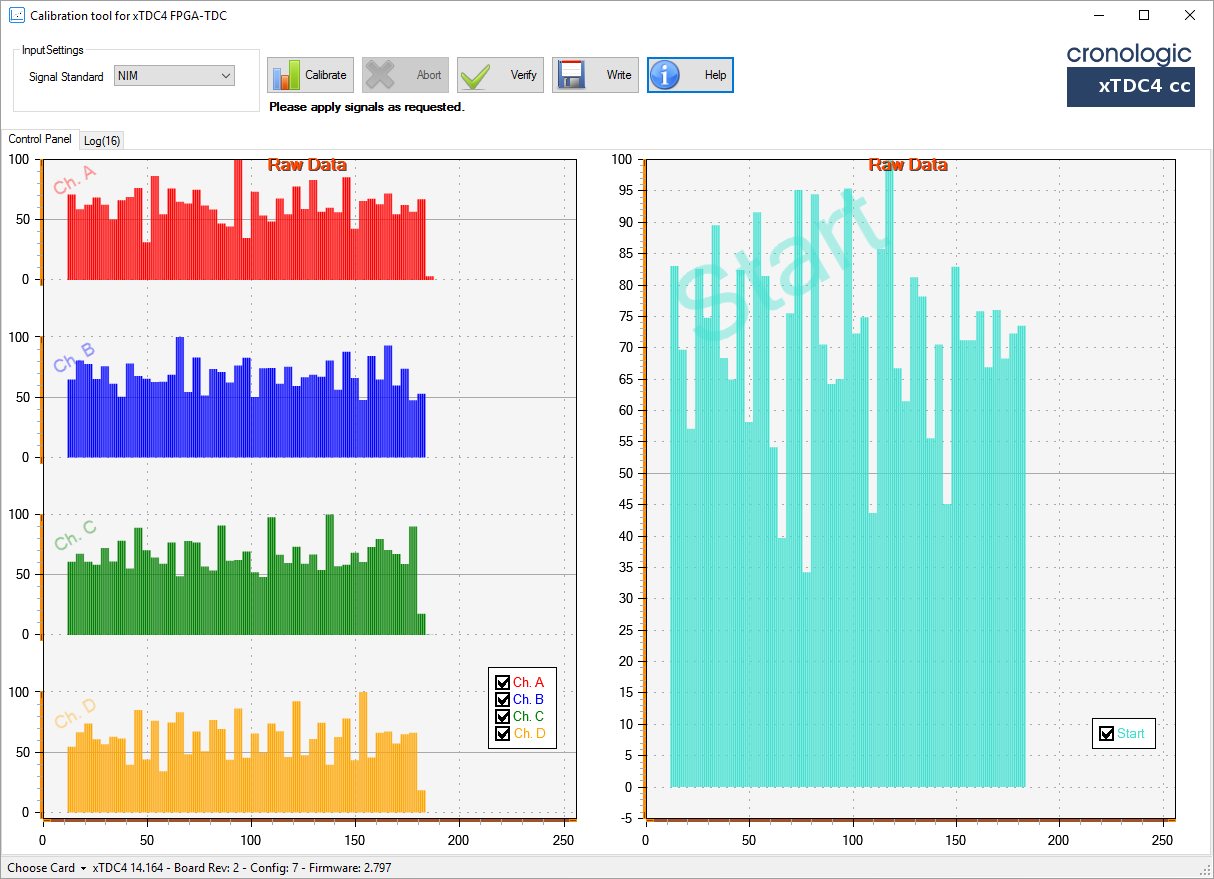
\includegraphics[width=\textwidth]{figures/XTDC4_Calibration.png}
    \caption{The \deviceName\ Carry Chain TDC calibration tool.\label{fig:calibTool}}
\end{center}
\end{figure*}
}